\newpage
\section{Grundlagen}
\label{sec:Grundlagen}
Das folgende Kapitel stellt die theoretischen und technologischen Grundlagen vor, die für das Verständnis und die Umsetzung dieser Arbeit erforderlich sind.
Es beginnt mit einer Einführung in die Industrie 4.0, und vermittelt ein grundlegendes Verständnis für das Konzept des digitalen Zwillings.
Anschließend werden die Struktur und Funktion der \acs{aas} sowie die Rolle des \acs{dpp} erläutert.
Den Abschluss bilden die technologischen Voraussetzungen für die praktische Umsetzung, darunter beispielsweise die Open-Source-Plattform Eclipse BaSyx oder der Kommunikationsstandard \ac{opcua}.
\subsection{Industrie 4.0}
% Nach der dritten industriellen Revolution, die vor allem durch den Einsatz elektronischer Systeme sowie der Informations -und Kommunikationstechnologie zur Automatisierung gekennzeichnet ist, vollzieht sich aktuell ein neuer technologischer Wandel, die vierte industrielle Revolution.
% Besser bekannt als Industrie 4.0, beschreibt sie die umfassende Vernetzung und Integration der physischen mit der digitalen Welt durch den Einsatz Cyber-physischer Systeme.

Der Begriff Industrie 4.0 wurde erstmals im Jahr 2011 im Rahmen eines von der deutschen Bundesregierung initiierten Zukunftsprojekts eingeführt, das auf die Förderung der Informatisierung in der industriellen Fertigung/Produktion abzielt.
Angestrebt wird eine Stärkung der Wettbewerbsfähigkeit der deutschen Industrie sowie eine Verbesserung der Marktposition deutscher Unternehmen im globalen Wettbewerb.

Industrie 4.0 steht dabei für die vierte industrielle Revolution und beschreibt die umfassende digitale Transformation industrieller Wertschöpfungsprozesse. 
Im Zentrum steht die intelligente Vernetzung von Menschen, Maschinen und Produkten über moderne digitale Kommunikationsnetzwerke, durch die eine weitreichende Integration der physischen mit der digitalen Welt ermöglicht wird.

Zur besseren Einordnung von Industrie 4.0 ist ein Blick auf die vorangegangenen industriellen Revolutionen hilfreich.
Die Industrialisierung begann bereits Mitte des 18. Jahrhunderts in Großbritannien und breitete sich von dort an weltweit aus. 
Mit der Entwicklung der ersten Dampfmaschine setzte die erste industrielle Revolution ein. 
Sie ermöglichte erstmals die Mechanisierung der Fertigung durch den Einsatz von Arbeits- und Kraftmaschinen. 
Dadurch konnten manuelle Tätigkeiten zunehmend durch Maschinenkraft ersetzt werden, insbesondere in der Textil-, Eisen- und Stahlindustrie, die zu den ersten Branchen gehörten, die von dieser Entwicklung profitierten.

Die zweite industrielle Revolution setzte gegen Ende des 19. Jahrhunderts ein und war maßgeblich durch den flächendeckenden Einsatz von Elektrizität geprägt. 
Mit der Erfindung elektrischer Antriebe und des Verbrennungsmotors konnten Maschinen nun auch dezentral betrieben werden. Sie waren nicht länger auf zentrale Kraftquellen wie Dampfmaschinen angewiesen. 
Dies ermöglichte eine flexiblere Gestaltung von Produktionsstätten und führte zur Entwicklung einer arbeitsteiligen Massenproduktion mithilfe von Fließ- und Förderbändern.

Ausgehend von dem deutschen Wirtschaftswunder in den sechziger Jahren des 20. Jahrhunderts entstand in den folgenden Jahrzehnten die dritte industrielle Revolution.
Diese zeichnet sich vor allem durch den Einsatz elektronischer Systeme sowie der Informations- und Kommunikationstechnologie zur Automatisierung aus und ist noch bis heute wirksam.

Aufbauend auf den vorangegangenen industriellen Revolutionen strebt die vierte industrielle Revolution eine tiefgreifende Transformation industrieller Produktionsprozesse an. 
Im Fokus steht dabei die Vernetzung von Systemen, die über moderne Internettechnologien miteinander kommunizieren.
Ziel dieser Entwicklung ist es, die industrielle Wertschöpfung deutlich flexibler und effizienter zu gestalten sowie eine stärkere Individualisierung von Produkten zu ermöglichen. 
\cite{Industrie4.0ProduktionAutomatisierung}\cite{EinführungundUmsetzungI4.0}

Trotz der weiten Verbreitung des Begriffs Industrie 4.0 mangelt es in der Literatur und Forschung an einer einheitlichen Definition.
Vor diesem Hintergrund nimmt insbesondere die Plattform Industrie 4.0 \cite{plattform_i40} eine zentrale Rolle in Deutschland ein. 
Dabei handelt es sich um eine gemeinsame Initiative des Bundesministeriums für Wirtschaft und Energie, des Bundesministeriums für Forschung, Technologie und Raumfahrt sowie führender Industrieverbände, Unternehmen, Forschungseinrichtungen und Gewerkschaften, darunter etwa der Verband Deutscher Maschinen- und Anlagenbau (VDMA), der Bundesverband Informationswirtschaft, Telekommunikation und neue Medien (Bitkom) und der \ac{zvei}.

Die Plattform ist maßgeblich an der inhaltlichen und strategischen Ausarbeitung der Industrie 4.0 beteiligt und leistet einen entscheidenden Beitrag zur Begriffsdefinition. 
Sie definiert Industrie 4.0 als
\glqq die vierte industrielle Revolution, einer neuen Stufe der Organisation und Steuerung der gesamten Wertschöpfungskette über den Lebenszyklus von Produkten.
Dieser Zyklus orientiert sich an den zunehmend individualisierten Kundenwünschen und erstreckt sich von der Idee, dem Auftrag über die Entwicklung und Fertigung, die Auslieferung eines Produkts an den Endkunden bis hin zum Recycling, einschließlich der damit verbundenen Dienstleistungen.
Basis ist die Verfügbarkeit aller relevanten Informationen in Echtzeit durch Vernetzung aller an der Wertschöpfung beteiligten Instanzen sowie die Fähigkeit aus den Daten den zu jedem Zeitpunkt optimalen Wertschöpfungsfluss abzuleiten. 
Durch die Verbindung von Menschen, Objekten und Systemen entstehen dynamische, echtzeitoptimierte und selbst organisierende, unternehmensübergreifende Wertschöpfungsnetzwerke, die sich nach unterschiedlichen Kriterien wie beispielsweise Kosten, Verfügbarkeit und Ressourcenverbrauch optimieren lassen \grqq~\cite[S. 8]{plattform_i40_definition}.

Die Definition der Plattform Industrie 4.0 verdeutlicht: Industrie 4.0 steht für einen grundlegenden Wandel in der industriellen Wertschöpfung.
Im Zentrum stehen dabei nicht nur neue technologische Möglichkeiten, sondern vor allem das Potenzial, Produktions- und Geschäftsprozesse flexibler, effizienter und nachhaltiger zu gestalten.
Durch die intelligente Vernetzung und die Nutzung von Echtzeitdaten enstehen selbstorganisierende Systeme, die auch über Unternehmensgrenzen hinweg kooperieren und tiefgreifende organisatorische Veränderungen erfordern.
Auf diese Weise werden nicht nur Qualität und Transparenz gesteigert, sondern auch Resourcen geschont und Kosten reduziert.
Insgesamnt trägt Industrie 4.0 somit nicht nur zur Verbesserung der Wirtschaftlichkeit bei, sondern leistet auch einen wichtigen Beitrag zur ökologischen Nachhaltigkeit.


% Obwohl Industrie 4.0 häufig als neuartiges Konzept dargestellt wird, basiert es im Kern auf Ideen, die schon seit mehreren Jahrzenten exisiteren.
% Bereits seit den 1980er-Jahren wurden mit Ansätzen wie dem Computer Integrated Manufacturing (CIM) oder der intelligenten Fabrik (Smart Factory) Strategien entwickelt, die auf eine computerintegrierte und automatisierte Produktion abzielen und dabei den Menschen mehr in den Hintergrund rücken.
% Allerdings scheiterten diese frühen Ansätze oft an den technische Möglichkeiten der damaligen Zeit, vor allem fehlte die Infrastruktur, Rechenleistung und Vernetzung.
% Erst mit dem technologischen Fortschritt, insbesondere der Einführung des Internetprotokolls V6 im Jahr 2012, wurde die Grundlage für eine globale, skalierbare Vernetzung von Maschinen, Produkten und Menschen im Sinne des Internet of Things geschaffen.
% Dies ermöglichte erstmals die Realisierung des Internet der Dinge (Internet of Things (IoT)), welches die technologische Basis für die Industrie 4.0 bildet.

\subsection{Künstliche Intelligenz}
% Künstliche Intelligenz ist eine Schlüsselkomponente der Industrie 4.0.
Mit der zunehmenden Vernetzung von Maschinen und Anlagen entstehen immer größere Datenmengen entlang von Produktionsprozessen.
Diese Daten bieten enorme Potenziale zur Optimierung industrieller Abläufe, beispielsweise zur Steigerung der Anlagenverfügbarkeit, zur Reduzierung von Ausschuss oder zur Verbesserug der Produktqualität.
Zudem erlauben intelligente Produkte, das Hersteller auch während der Nutzungsphase Informationen über den Einsatz und Zustand eines Produktes erhalten.
Auf Basis dieser lassen sich neue Dienstleistungen und Anwendungen entwickeln, wie etwa die vorrauschaunde Instandhaltung oder die dynamische Optimierung von Betriebsparametern.

Damit solche datengetriebenen Ansätze erfolgreich umgesetzt werden können, benötigt es leistungsfähige Technologien zur Analyse und Interpretation.
Genau hier setzt \acs{ki} an.
Insbesondere Methoden des maschinellen Lernens erlauben es, Zusammenhänge in großen Datenmengen zu erkennen, Zustände zu klassifizieren und sogar Vorhersagen über zukünftige Systementwicklungen zu treffen. \cite{KIEinführung} 
\acs{ki} nimmt somit eine zentralle Rolle innerhalb der Industrie 4.0 ein, indem sie einen echten Mehrwert aus den gesammelten Daten generiert.

Allgemein bezeichnet der Begriff \acs{ki} dabei eine Vielzahl von Methoden und Technologien, die es Computern ermöglichen, Aufgaben zu bewältigen, für die normalerweise menschliche Intelligenz erforderlich ist \cite{KIDefinition1}.
Dazu zählen insbesondere die Fähigkeit, aus Erfahrungen (Daten) zu lernen, Problemlösungen zu entwickeln sowie selbstständig Entscheidungen zu treffen \cite{KIDefinition2}.

Ein zentrales Teilgebiet der \acs{ki} ist das maschinelle Lernen.
Es umfasst Algorithmen, die selbstständig aus Daten lernen und darauf basierend Vorhersagen treffen können.
Im Gegensatz zu klassischen Computerprogrammen folgt das Programm keinem Lösungsweg. 
Stattdesen erkennt es Muster in den vorliegenden Daten und kann auf Grundlage dieser bestimmte Aufgaben ausführen \cite{MLDefinition}.
Aufgrund seiner zentralen Bedeutung für zahlreiche Anwendungen gilt maschinelles Lernen häufig auch als Schlüsseltechnologie der \acs{ki} \cite{MLSchlüsseltechnologie}. 

Grundsätzlich wird zwischen überwachtem Lernen (Supervised Learning) und unüberwachtem Lernen (Unsupervised Learning) unterschieden.
Beim überwachten Lernen wird ein Modell anhand eines Datensatzes trainiert, der sowohl Eingabewerte als auch die dazugehörigen Ziel- bzw. Ausgabewerte enthält.
Der Algorithmus lernt dabei, Zusammenhänge und Muster in den Daten zu erkennen, um daraus eine Funktion abzuleiten, die neue Eingaben korrekt vorhersagen kann.
Typische Anwendungsbereiche sind die Klassifikation (z. B. die Einteilung von Bildern in Kategorien) und die Regression (z. B. die Vorhersage numerischer Werte wie Temperatur oder Energieverbrauch).

Beim unüberwachtem Lernen hingegen wird ein Modell mit ungelabelten Daten trainiert, das heißt ohne vorgegeben Zielwerte. 
Der Algorithmus versucht selbstständig Strukturen oder Muster in den vorgegeben Daten zu finden.
Ein häufig eingesetztes Verfahren ist die Clusteranalyse, bei der ähnliche Datenpunkte zu Gruppen, sogenannten Clustern, zusammengefasst werden. 
Eine typische Anwendung ist beispielsweise die Anomalieerkennung, bei der Abweichungen von einem erwarteten Normalverhalten erkannt werden können.

Ein besonders leistungsfähiger Ansatz innerhalb des maschinellen Lernens ist das Deep Learning \cite{DLEinordnung}.
Es basiert auf künstlichen neuronalen Netzen, die in ihrer Struktur an das Verhalten von Neuronen im menschlichen Gehirn angelehnt sind.
Während klassische maschinelle Lernmodelle meist aus nur wenigen Schichten bestehen, kommen beim Deep Learning sogenannte tiefe neuronale Netze mit vielen hintereinandergeschachtelten Schichten zum Einsatz.
Diese ermöglichen das Erkennen hochkomplexer und abstrakter Zusammenhänge in großen Datenmengen, etwa bei der Bilderkennung oder der Sprachverarbeitung. \cite{DLDefinition}
Ein besonders aktuelles Beispiel für die Anwendung tiefer neuronaler Netzwerke ist die generative \acs{ki}. 
Sie beschäftigt sich mit der Erstellung neuer Inhalte wie Text oder Sprache. 
Dabei kommen verschiedene Methoden des Deep Learnings zum Einsatz, um aus großen Datenmengen zu lernen, wie neue Inhalte erzeugt werden können \cite{GenerativeKI}.

% \subsubsection{RAMI 4.0}
% Das \ac{rami} ist ein Leitfaden für die Industrie und dient als Hilfestellung um die digitale Transformation in einem Unternehmen systematisch umzusetzten.
% Es wird in der DIN SPEC 91345 \cite{RAMI4.0} standardisiert und soll helfen, die komplexen Anforderungen an die Industrie 4.0 für die Allgemeinheit verständlich zu machen.
% Das Modell ist als dreidimensionales Koordinatensystem konzipiert und umfässt die Achsen ... .


% \begin{figure}[htbp]
%     \centering
%     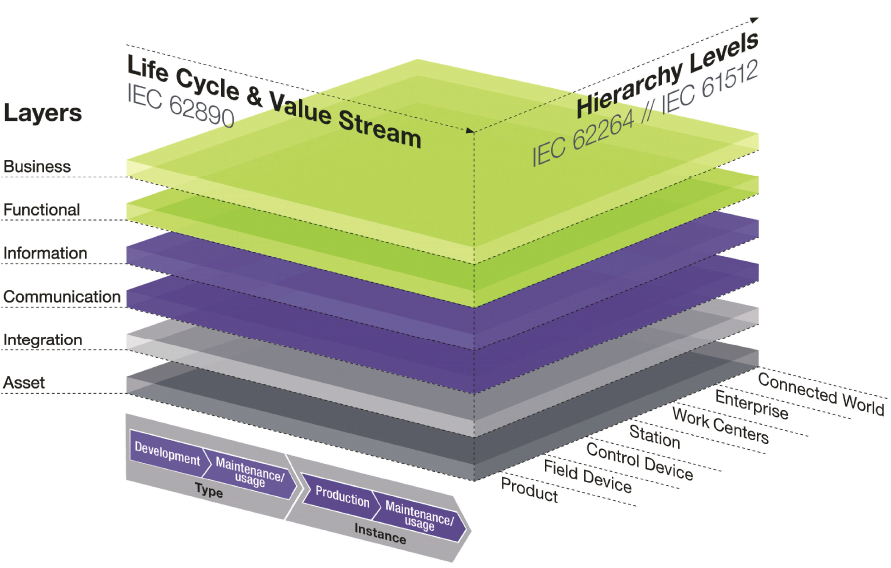
\includegraphics[width=0.8\textwidth]{Bilder/RAMI.PNG}
%     \caption{Referenzarchitekturmodell Industrie 4.0 (RAMI 4.0)}
%     \label{fig:klassifizierungDT}
% \end{figure}

\newpage
\subsection{Digitaler Zwilling}
\label{sec: DT}
Digitale Zwillinge gelten als eine der Schlüsseltechnologien der Industrie 4.0.
Als digitales Gegenstück eines physischen Objekts, sei es eine Maschine ein Produkt oder eine komplette Anlage, bilden sie dessen Zustand, Verhalten und Leistung virtuell ab.
Dadurch ermöglichen sie eine konsistenete Erfassung von Daten, das Simulieren von Prozessen und das frühzeitige Erkennen von Optimierungspotenzialen.

Das Konzept selbst wurde erstmals von Michael Grieves im Jahr 2003 in einer Präsentation zum \ac{plm} vorgestellt. 
Grieves definierte drei grundlegende Komponenten \cite{DTGrieves} , die zusammen das Informationsmodell des digitalen Zwilling bilden:
\begin{itemize}
    \item ein reales Objekt in der physischen Welt,
    \item ein digitales Abbild dieses Objekts in einem virtuellen Raum, sowie
    \item eine Schnittstelle, die den Informationsfluss zwischen diesen beiden ermöglicht.
\end{itemize}

Auf Basis des von Grieves entwickelten Informationsmodells hat sich der Begriff des digitalen Zwillings kontinuierlich weiterentwickelt.
Aufgrund verschiedener Fachgebiete und inkonsistenter Definitionen haben sich in der Vergangenheit allerdings eine Vielzahl unterschiedlicher Ausprägungen des Begriffs gebildet.
Diese unterscheiden sich insbesondere in der Tiefe der Datenintegration zwischen dem physischen Objekt und seinem virtuellen Abbild.
Während ein einfacher digitaler Zwilling lediglich ein einfaches Modell mit statischen Daten ist, ermöglichen fortgeschrittene Zwillinge einen bidrektionalen Datenaustausch zwischen physischem und virtuellem Objekt. 

Für ein besseres Verständnis und zur tieferen Klassifizierung ist es zunächst hilfreich, zwischen Typen und Instanzen des digitalen Zwillings zu unterscheiden.
Typen sind allgemeine Abbilder, die grundlegende Eigenschaften und Verhaltensmodelle einer Produktgruppe beschreiben. 
Sie können mit einer Klasse in der Softwarentwicklung verglichen werden, die als Vorlage für konkrete Instanzen dienen.
Typen können beispielsweise einen bestimmten Maschinentyp hinsichtlich Aufbau, Stuktur oder Schnittstellen beschreiben, ohne dabei Bezug zu einer einzelnen physischen Maschine zu nehmen.
Instanzen wiederrum sind einzigartig, und beschreiben ein konkretes Produkt, etwa eine Maschine, die einzigartig über eine Seriennummer identifizierbar ist.
Häufig sind Instanzen Aussprägungen eines Types mit einer Verbindung zu einem realen Objekt, wodurch beispielsweise die Überwachung des Zustands einer Produktionsanlage ermöglicht wird.
Analog zur Softwarentwicklung können diese als instanziiertes Objekt einer Klasse gesehen werden. \cite{ZEISS}

Je nach Art des Informationsflusses sowie dem Grad der Ausprägung der Verbindung zur realen Welt werden Instanzen digitaler Zwillinge häufig in drei Kategorien eingeteilt: das digitale Modell, den digitalen Schatten und den digitalen Zwilling \cite{ClassificationDT}.
Obwohl diese Begriffe im allgemeinen Sprachgebrauch oft synonym verwendet werden, unterscheiden sie sich deutlich hinsichtlich ihrer Funktion und Kopplung zum realen Objekt.

Digitale Modelle sind statische Abbilder physischer Objekte, haben jedoch keine Verbindung zu diesen. 
Oft werden sie zur Veranschauclichung oder Konstruktion genutzt, wie zum Beispiel ein 3D-Modell einer Maschine.
Zwar können reale Daten, wie etwa Maße oder Materialeigenschaften einer Anlage oder Maschine in ein solches Modell integriert werden, allerdings erfolgt die Eingabe dabei immmer manuell.
Änderungen an dem realen Objekt werden nicht automatisch aktualisiert und bleiben somit ohne Einfluss auf das digitale Modell.

Der digitale Schatten ergänzt das digitale Modell um eine unindirektionale Verbindung zum realen Objekt.
Dabei fließen Daten des physischen Objekts meist in Echtzeit über zum Beispiel geeignete Sensoren zum digitalen Objekt.
Der Schatten bildet den aktuellen Zustand des Objekts ab, hat aber keine Rückkoplung zu diesem.
Ein typisches Beispiel für einen digitalen Schatten wäre das Condition Monitoring, wobei der Zustand einer Maschine mit geeigneten Sensoren abgebildet wird.

Mit einer aktiven Rückkoplung zum realen Objekt wird der digitale Schatten zum digitalen Zwilling.
Es entsteht eine Feedback-Schleife, die es dem virtuellen Objekt erlaubt, Einfluss auf das reale System zu nehmen.
Eine Übersicht der drei Kategorien zeigt Abbildung \ref{fig:klassifizierungDT}. 
% Quelle: file:///C:/Users/Heinke/Documents/Bachelorarbeit/02%20Literatur/Digitaler_Zwilling/Klassifizierung_DT.pdf
\vspace{-0.5em}
\begin{figure}[htbp]
    \centering
    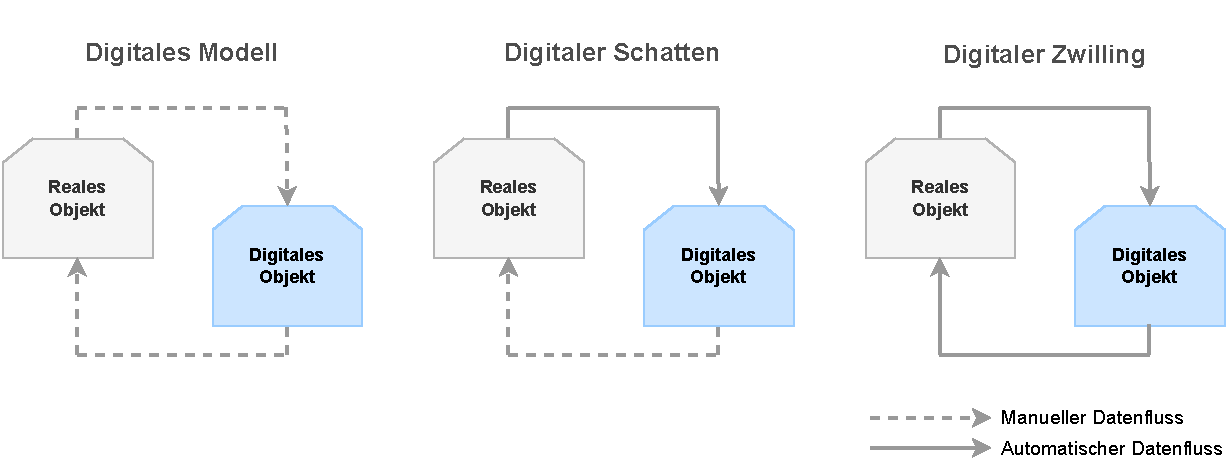
\includegraphics[width=1\textwidth]{Bilder/klassifizierung_DT.pdf}
    \caption[Klassifizierung des digitalen Zwillings]{Klassifizierung des digitalen Zwillings (in Anlehnung an \cite{ClassificationDT})}
    \label{fig:klassifizierungDT}
\end{figure}
\vspace{-0.5em}

Im industriellen Umfeld werden digitale Zwillinge in vielen unterschiedlichen Bereichen genutzt.
Sie kommen entlang des gesamten Lebenszyklus eines Assets zum Einsatz, von der Entwicklung über die Produktion bis hin zum Betrieb und der Wartung.%
\pagebreak 
~Dabei ist jedoch zu beachten, das in der Praxis häufig auch digital Modelle oder digitale Schatten als digitale Zwillinge bezeichnet werden, obwohl sie technisch gesehen nicht alle Merkmale eines echten digitalen Zwillings aufweisen und somit ebenfalls nicht ihr volles Potenzial entfalten.

Bereits bei der Entwicklung von Produkten können digitale Zwillinge einen erheblichen Vorteil bieten. 
Indem bereits frühzeitig digitale Modelle oder Simulationen eingesetzt werden, entfällt die Notwendigkeit physischer Prototypen, was Entwicklungszeiten und Kosten deutlich senken kann. Während der Produktion ermöglichen sie eine durchgängige Überwachung, Analyse und Optimierung von Fertigungsprozessen durch die Integration von Echtzeitdaten.
Sie unterstützen die virtuelle Inbetriebnahme von Maschinen und dienen als Grundlage für die vorausschauende Wartung (Predictive Maintenance), wodurch Stillstandzeiten einer Maschine reduziert werden können.
Nicht zuletzt dienen digitale Zwillinge als zentrale Datenplattform, in der alle relevanten Informationen aus verschiedenen Datenquellen gebündelt werden.
Sie bilden somit eine konsistente Datenbasis und können beispielsweise bei dem Entwicklungsprozess eines Produktes helfen. \cite{DTForSmartManufacturing}

Die Implementierung digitaler Zwillinge erweist sich in der Praxis jedoch oftmals als sehr anspruchsvoll.
Eine zentrale Herausforderung ist die fehlende Interoperabilität zwischen verschiedenen IT-Systemen.
Sowohl innerhalb eines Unternehmens als auch unternehmensübergreifend bilden sich dadurch häufig voneinander isolierte Datenbestände, die nicht systemübergreifend nutzbar sind.
Solche sogenannten Informationssilos können die Umsetzung eines konsistenten digitalen Zwillings erheblich erschweren, da die relevanten Informationen und Daten zunächst aus unterschiedlichen Systemen wie \ac{erp}, \ac{mes} oder \ac{cad} zusammengeführt werden müssen.

Hinzu kommt, das diese Daten oftmals in unterschiedlichen, nicht standardisierten Formaten vorliegen, was eine automatisierte Integration zusätzlich erschwert.
Diese Problematik zeigt sich nicht nur innerhalb einzelner Unterhnehmen, sondern auch entlang der gesamten Wertschöpfungskette, etwa wenn verschiedene Akteure einer Lieferkette heterogene Datenformate und proprietäre Austauschprotokolle verwenden.
Ein digitaler Zwilling, der in einem Unternehmen A erstellt wurde, kann dadurch von einer Anwendung oder einem weitern digitalen Zwilling eines Unternehmens B nicht ohne Weiteres intepretiert oder verwendet werden.
Es ist daher essenziell, digitale Zwillinge in einem interoperablen Format bereitzustellen, um eine einheitliche Interpretation und Nutzung auch über Unternehmensgrenzen hinweg zu ermöglichen.
\cite{DTandAASConceptsInI4.0}

\newpage
\subsection{Asset Administration Shell}
\label{chap:AAS}
% Das \ac{rami} ist ein Leitfaden für die Industrie und dient als Hilfestellung um die digitale Transformation in einem Unternehmen systematisch umzusetzten.
% Es wird in der DIN SPEC 91345 \cite{RAMI4.0} standardisiert und soll helfen, die komplexen Anforderungen an die Industrie 4.0 für die Allgemeinheit verständlich zu machen.
% Das Modell ist als dreidimensionales Koordinatensystem konzipiert und umfässt die Achsen ... .

Die \acs{aas} - deutsch Verwaltungsschale - ist eine Schlüsselkomponente innerhalb des \ac{rami} \cite{RAMI4.0} und bildet die Grundlage für die Umsetzung und Entwicklung interoperabler digitaler Zwillinge im industriellen Umfeld.
Sie wurde maßgeblich von der Plattform Industrie 4.0 entwickelt und erstmals im Jahr 2016 als Teil von \acs{rami} vorgestellt.
Seit ihrer Einführung wurde die \acs{aas} kontinuierlich weiterentwickelt und ist mittlerweile in der internationalen Norm IEC 63278-1 \cite{AASIEC63278} standardisiert.
% Darin wird die AAS als "strukturierte, standardisierte digitale Repräsentation eines Assets" definiert.

Seit 2020 wird die Umsetzung und Weiterentwicklung der \acs{aas} von der \acs{idta} \cite{IDTA} organisiert und gesteuert.
Ziel der Organisation ist es, den digitalen Zwilling auf Basis der \acs{aas} zu standardisieren und in Form von Open-Source-Softwarelösungen in das industrielle Umfeld zu integrieren.
Die \acs{aas} wird dabei in mehreren Spezifikationen der \acs{idta} dokumentiert und beschrieben.
Aktuell bildet die \acs{aas}-Version 3 den neuesten Entwicklungsstand und ist ebenfalls die Basis für diese Arbeit.
% evtl die Quelle wenn gut https://www.zvei.org/themen/start-der-industrial-digital-twin-association-idta

Die \acs{aas} repräsentiert ein Asset digital, indem sie alle relevanten Daten, Eigenschaften und Funktionen über den gesamten Lebenszyklus hinweg in strukturierter und standardisierter Form bereitstellt. 
Sie fungiert somit als digitales Gegenstück eines realen Objekts - also als digitaler Zwilling.
Die Informationen sind in sogenannten Submodellen organisiert, die jeweils spezifische Aspekte eines Assets abbilden.
Dabei kann es sich sowohl um physische Assets (z.B. Maschinen, Anlagen) als auch um virtuelle Assets (z.B. Software, Konzepte) handeln. 
Eine \acs{aas} ist dabei stets einem Asset zugeordnet und global eindeutig identifizierbar. 
Durch die Kombination eines Assets mit seiner \acs{aas} entsteht eine sogenannte Industrie 4.0-Komponente (siehe Abbildung \ref{fig:Industrie4Komponente}).

% Durch die standardisierte Struktur bildet die Verwaltungsschale die Grundlage für einen einheitlichen Informationsaustausch über System -und Unternehmensgrenzen hinweg.
% Verwaltungsschalen repräsentieren immer genau ein Asset und müssen global eindeutig identifizierbar sein.
% In der Industrie können Assets physische Objekte, wie eine Anlage oder eine Maschine sein oder aber auch virtuelle Elemente wie Software oder eine Idee.
% In RAMI 4.0 wird davon ausgegangen, das Assets immmer einen konkreten Nutzen für ein Unternehmen bzw. eine Organisation bieten.
\vspace{1em}
\begin{figure}[htbp]
    \centering
    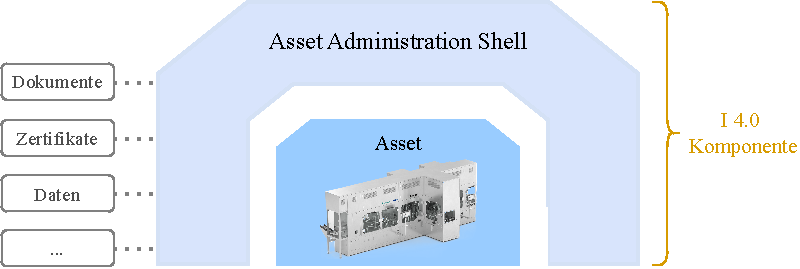
\includegraphics[width=1\textwidth]{Bilder/I4Komponente/I4KomponenteNeu.pdf}
    \caption[Industrie 4.0 Komponente]{Industrie 4.0 Komponente (Bildbestandteil: \cite{robocellLogo})}
    \label{fig:Industrie4Komponente}
\end{figure}

\subsubsection{Aufbau und Struktur}
Analog zur in Kapitel \ref{sec: DT} beschriebenen Unterscheidung von Typen und Instanzen digitaler Zwillinge unterscheidet auch die \acs{aas} zwischen diesen beiden Ausprägungen.
Während Typ-\acs{aas} allgemeine Merkmale und Strukturen eines Produkttyps beschreiben, sind Instanz-\acs{aas} konkreten physischen oder virtuellen Objekten zugeordnet und enthalten spezifische Informationen wie Seriennummer, Zustand oder Standort.

Bestimmte Aspekte eines Assets werden gemäß der Spezifikation des Metamodells der AAS \cite{SpezifikationPart1} in verschiedenen Submodellen verwaltet.
Man kann sich dies wie ein Schubladensystem vorstellen, wobei jede Schublade einen bestimmten Bereich des Assets abdeckt, beispielsweise die technischen Stammdaten, das Typenschild, Wartungsinformationen oder Zustandswerte einer Maschine.
Die Auswahl und Struktur der Submodelle ist domänenspezifisch und hängt stark vom konkreten Asset bzw. Anwendungsfall ab. 
Dabei kann eine \acs{aas} beliebig viele Submodelle enthalten, die bei Bedarf auch erweitert werden können. 

Die Daten innerhalb eines Submodells werden in verschiedenen Submodellelementen strukturiert.
Diese umfassen Dateneigenschaften, Operationen sowie weitere Sutrukturellemente die für eine umfassende Beschreibung eines digitalen Modells eines Assets erforderlich sind.
So erlaubt beispielsweise das RelationshipElement die Modellierung von Beziehungen oder das ReferenceElement die Referenzierung von internen oder externen Inhalten.
Das vermutlich am häufigsten verwendete Datenelement ist das Submodellelement Property.
Es lässt sich mit einer Variablen aus der Softwareentwicklung vergleichen, da es einfache Merkmale wie etwa einen Namen oder eine Seriennummer repräsentiert und dabei über einen definierten Datentyp wie String, Integer oder Boolean verfügt.

Wichtig ist, sowohl die \acs{aas} selbst als auch ihre Submodelle müssen global eindeutig identifizierbar sein.
Dies wird durch die Verwendung von eindeutigen Identifikatoren (\acsp{id}) der Klasse Identifiable wie einer URI (Uniform Resource Identifier) oder \acs{irdi} (International Registration Data Identifier) sichergestellt.
Für die Elemente innerhalb eines Submodells ist eine lokale Kennung ausreichend. 
Dies erfolgt in der Regel anhand einer idShort der Klasse Referable, die einen kurzen, aussagekräftigen Namen enthält.

Zur besseren Veranschaulichung der zugrunde liegenden Struktur der \acs{aas} dient Abbildung \ref{fig:MetamodellAAS}, die eine vereinfachte Darstellung des Metamodells zeigt.

% Neben Properties spielt zudem das Submodellement File eine besonders wichtige Rolle. Es ermöglicht das Einbetten oder Referenzieren von Dateien in die \acs{aas}. 
% Dabei werden gängige Dateiformate wie PDF, JPG oder STEP unterstützt, was besonders für technische Dokumentationen oder \acs{cad}-Modelle von Bedeutung ist.
% Neben diesen Datenelementen existieren noch weitere Submodellelemente, die spezifische Funktionen ermöglichen. 
% So erlaubt beispielsweise das RelationshipElement die Modellierung von Beziehungen oder das ReferenceElement die Referenzierung von internen oder externen Inhalten.
% Zur besseren Veraunschaulichung des zugrundeliegenden Metamodells wird dieses nachfolgend in einer vereinfachten Form dargestellt.

\newpage
\begin{figure}[htbp]
    \centering
    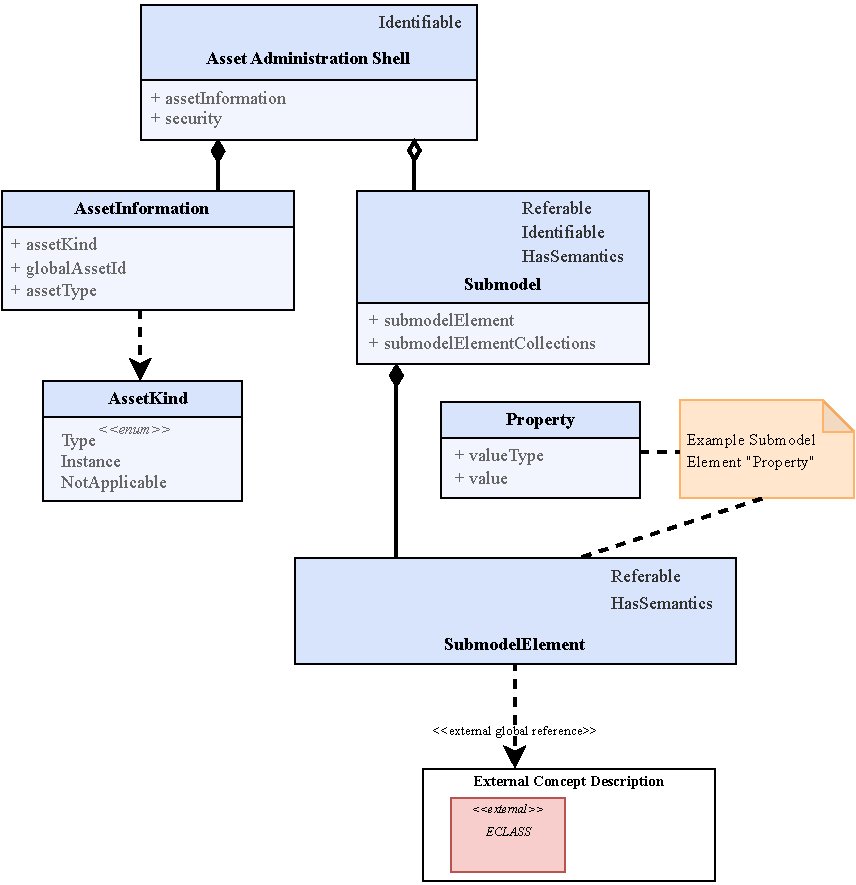
\includegraphics[width=1\textwidth]{Bilder/Metamodell/MetamodellFarbig.pdf}
    \caption[Vereinfachtes Metamodell der \acs{aas}]{Vereinfachtes Metamodell der \acs{aas} (in Anlehnung an \cite{SpezifikationPart1})}
    \label{fig:MetamodellAAS}
\end{figure}

Eine eindeutige semantische Beschreibung aller Submodelle und ihrer Elemente ist essenziell, um ein einheitliches Verständnis zwischen unterschiedlichen Systemen sicherzustellen.
Hierfür wird die sogenannte semanticId der Klasse HasSemantics verwendet, welche eine semantische Referenz enthält.
Diese verweist entweder auf einen externen Standard oder auf eine lokale \ac{cd}, die direkt in der \acs{aas} eingebettet ist.
Ein häufig verwendeter externer Standard ist zum Beispiel ECLASS, welcher auf der Norm IEC 61360 \cite{ECLASSIEC61360} basiert.

Zur formalen Beschreibung solcher Concept Descriptions stellt die \acs{idta} standardisierte Data Specification Templates gemäß der Norm IEC 6130 \cite{SpezifikationPart3a} bereit.
Diese liefern ein strukturiertes Modell zur Beschreibung technischer Merkmale.
Darin enthalten sind unter anderem Definitionen, Einheiten, Wertebereiche, zulässige Werte sowie externe Referenzen, die bestimmten Submodellen oder Submodellelementen zugeordnet werden können.
% Dadurch wird ein gemeinsames semantisches Verständnis zwischen unterschiedlichen Systemen ermöglicht.

%Fehlt die semantische Beschreibung, so kann es schnell zu Missverständnissen kommen.
%Liegt beispielsweise ein einfacher Wert 25 vor, ist ohne weitere Informationen unklar, was gemeint ist. 
%Es könnte sich um 25 Euro, 25 Meter oder 25 Grad Celsius handeln.
%Erst durch die zugehörige semantische Beschreibung, in der die Einheit und Bedeutung definiert werden, wird der Wert eindeutig interpretierbar. 

Um die Erstellung von Submodellen zu erleichtern und gleichzeitig Interoperabilität zu gewährleisten, stellt die \acs{idta} standardisierte Submodellvorlagen - sogenannte \acp{smt} - zur Verfügung.
Diese Templates decken eine Vielzahl industrieller Anwendungsfälle ab und werden kontinuierlich weiterentwickelt und ergänzt.
Die bereits verfügbaren Templates enthalten unteranderem Submodelle wie das digitale Typenschild oder den \ac{cf}.
Alle Eigenschaften innerhalb dieser Vorlagen werden dabei in Verbindung mit dem ECLASS-Standard einheiltich semantisch beschrieben.
Diese Templates könen über ein zentrales Repository \cite{idtaTemplates} bezogen werden und bilden die Basis für eine interoperable semantische Datenstruktur.

\subsubsection{Informationsaustausch}
Der Austausch von Informationen über die \acs{aas} kann auf unterschiedliche Weise erfolgen.
Die einfachste Möglichkeit besteht im Dateiaustausch. Hierfür wurden speziell für die \acs{aas} sogenannte AASX-Dateien \cite{SpezifikationPart5} entwickelt, die den einfachen Austausch statischer \acs{aas} (Typ-1-\acs{aas}) ermöglichen.
Dabei werden sämtliche Daten, Beziehungen, Strukturen sowie zugehörige Dateien der \acs{aas} serialisiert und in ein AASX-ZIP-Dateiformat gespeichert. 
Diese Datei kann anschließend über ein digitales Medium, etwa per E-Mail oder eine Cloud-Plattform, weitergegeben werden. 

Eine Typ-2-\acs{aas} hingegen wird von einer Laufzeitumgebung gehosted, wodurch ein direkter und dynamischer Zugriff auf ihre Inhalte ermöglicht wird. 
Die Spezifikitation Part 2: Aplication Programming Interfaces \cite{SpezifikationPart2} beschreibt hierfür nicht nur standardisierte Schnittstellen, sonder auch ein ganzheitliches System für das Verwalten, Bereitstellen und Auffinden der \acs{aas}.
Repositories dienen dabei als zentraler Speicherort für die Inhalte einer \acs{aas}, einschließlich ihrer Submodelle und Concept Descriptions.
Die Aufgabe der Verwaltung und Registrierung übernehmen sogenannte Registries.
Sie ermöglichen das systemweite Auffinden von \acs{aas} und stellen sicher, dass diese eindeutig referenzierbar sind.

Ergänzend dazu bieten Discovery Services eine erweiterte Suchfunktionalität, indem sie Beziehungen verschiedener Entitäten mittels verschiedener Schlüsselwertpaare speichern.
Eine \acs{aas} kann so zum Beispiel logisch mit einer Asset-\acs{id} verknüpft werden und somit schnell innerhalb komplexer Systeme identifiziert werden.
Der Zugriff auf diese Systeme bzw. ihrer Inhalte wird in Form von Schnittstellen standardisiert, wodurch eine hohe Interoperabilität gewährleistet wird.
Ein besonderer Fokus liegt dabei auf der Nutzung von \ac{http} gemäß dem \acs{rest}-Architekturstil (Representational State Transfer), der eine strukturierte Kommunikation über Methoden wie GET, POST, PUT oder DELETE ermöglicht.

Die fortschrittlichste Form des Informationsaustausches stellt die Peer-to-peer Kommunikation dar, bei der I4.0-Komponenten (Typ-3-\acs{aas}) eigenständig über die I4.0-Sprache miteinander kommunizieren.

\subsubsection{Sicherheit}
\label{sec: Sicherheit}
Gerade wenn Informationen aus der \acs{aas} über die Grenzen des eigenen Unternehmens hinweg bereitgestellt werden, ist es besonders wichtig, dass die enthaltenen Daten geschützt sind. 
Die neueste Spezifikation Part 4: Security \cite{SpezifikationPart4} der \acs{idta} liefert hierfür die technische und konzeptionelle Grundlage.
Sie beschreibt, wie Zugriffe auf Daten in der \acs{aas} sicher gesteuert werden können, insbesondere in vernetzten Umgebungen wie Datenräumen.

Zum Einsatz kommen dabei Dienste wie ein Identity Provider zur Authentifizierung oder ein Policy Service zur Durchsetzung von Richtlinien.
Die Sicherheit wird dabei mithilfe eines attributbasierten Zugriffsmodells (\ac{abac}) gewährleistet.
Bei jeder Anfrage auf bestimmte Objekte innerhalb der \acs{aas} wird dabei anhand verschiedener Merkmale (Attribute) geprüft, ob ein Zugriff erlaubt ist.
Dazu zählen sogenannte Subjektattribute (also wer die Anfrage stellt), Objektattribute (z.B. welches Submodell, welche Property oder welches Submodellelement betroffen ist), die gewünschte Aktion (z.B. Lesen oder Schreiben) sowie kontextbezogene Bedingungen (z.B. Zeitpunkt der Anfrage oder Zustand des Systems).

Die zur Prüfung notwendigen Informationen liefert in der Regel ein Token, das vom Identity Provider bereitgestellt wird. Die Spezifikation sieht hierfür die Nutzung sogenannter \acp{jwt} vor.
Die Attribute werden schließlich von dem Policy Service mit den dort hinterlegenen Zugriffsrichtlinen abgeglichen und basierend darauf eine Zugriffsentscheidung getroffen.
Ein besonderer Vorteil des \acs{abac}-Modells liegt dabei in seiner hohen Flexibilität. Rollen können ebenfalls als Attribute behandelt werden, wodurch sich auch problemlos rollenbasierte Zugriffskonzepte (RBAC) umsetzen lassen. 

Die beschriebenen Kontrollmechanismen lassen sich nicht nur auf die Inhalte der \acs{aas} selbst, sondern insbesondere auch auf die Schnittstellen von Registries und Repositories anwenden.
So kann beispielsweise sichergestellt werden, das nur authorisierte Systeme Zugriff auf ein bestimmtes Submodell erhalten oder nur bestimmte Nutzergruppen neue \acs{aas}-Instanzen registrieren können.
Diese Sicherheits-Konzepte sind jedoch noch%
\pagebreak
~vergleichsweise neu und müssen in der Praxis erst noch weiter erprobt werden.
Erste Referenzimplementierungen liegen zwar bereits häufig schon in Form rollenbasierter Zugriffskontrollen vor, eine vollständige Integration des \acs{abac}-Ansatzes steht jedoch noch aus.


\subsection{Digitaler Produktpass}
Der \acs{dpp} ist ein zentrales Instrument der Europäischen Union zur Umsetzung einer nachhaltigen, digitalen Transformation. 
Ziel ist es, die Transparenz über ökologische Merkmale von Produkten wie verwendete Materialien, Recylcebarkeit oder die CO\textsubscript{2}-Bilanz deutlich zu verbessern.
Hierzu müssen produktspezifische Daten über den gesamten Lebenszyklus hinweg aufgezeichnet und in einem menschen -und maschinenlesbarem Format bereitgestellt werden. \cite{DPPEinführung}
Langfristig soll dies zu einer Kreislaufwirtschaft und digitalen Wirtschaft innerhalb der EU führen.

Das Konzept des \acs{dpp} wurde erstmals im Rahmen des European Green Deal von der Europäischen Kommission im Jahr 2019 vorgestellt \cite{GreenDeal}.
Im Zuge der Ökodesign-Verordnung (\ac{espr}) \cite{ESPR} wird er aktuell als verpflichtendes Mittel für zahlreiche Produktgruppen eingeführt.
Als erste konkrete Anwendung wird der \acs{dpp} erstmals im Jahr 2027 für Batterien verpflichtend.
Weitere Produktkategorien, darunter auch die Elektroindustrie und der Maschinen -und Anlagenbau werden in den nächsten Jahren folgen.

Die Bereitstellung der Produktpässe erfolgt gemäß den Anforderungen der \acs{espr} in elektronischer Form. 
Dabei müssen diese untereinander interoperabel kommunizieren können.
Je nach Art der Information werden verschiedene Zugriffsrechte für unterschiedliche Interessengruppen eingeführt. 
Damit soll der Schutz von geistigem Eigentum sichergestellt werden.
Die Daten sollen dabei über einen zentralen Server bzw. ein Registry verwaltet werden, worin die verschiedenen \acsp{dpp} gespeichert bzw. registriert werden.
\cite{CIRPASS}

Während die regulatorischen Rahmenbedingungen mehr oder weniger final ausgearbeitet sind, bleibt die Frage der konkreten technologischen Umsetzung.
Eine dezentrale Lösung bildet der von der \acs{zvei} vorgestellte digitale Produktpass für Industrie 4.0 (\acs{dpp40}) \cite{DPP40}.
Dieser basiert auf zwei etablierten Standards. 
Zum Einen das digitale Typenschild, und zum Anderen die \acs{aas} (siehe auch Kapitel~\nameref{chap:AAS}).
Das digitale Typenschild ermöglicht, gemäß der Norm IEC 61406 \cite{TypenschildIEC61406-1}, die eindeutige Identifikation von Produkten über eine einzigartige Asset-\acs{id}.
Typischerweise wird diese in Form eines maschinenlesbarem Links oder QR-Codes an einem Produkt angebracht, die direkt zu dem zugehörigen \acs{dpp} führt.

Organisiert werden die Daten im \acs{dpp40} in verschiedenen Submodellen der \acs{aas}. 
Standardisierte Teilmodelle wie das digitale Typenschild, Dokumentationen oder der \ac{pcf} helfen bei der Umsetzung der im \acs{dpp} geforderten Daten.
Darüber hinaus können auch zusätzliche, nicht verpflichtende Informationen integriert werden, sofern sie für bestimmte Stakeholder einen Mehrwert bieten.
Der Zugriff auf die Daten ist über ein webbasiertes Portal vorgesehen. 

Verschiedene Interessengruppen erhalten dabei unterschiedliche Zugriffsrechte. 
Hierfür werden bestimmmte Submodelle gezielt für unterschiedliche Gruppen freigegeben oder eingeschränkt.
Während beispielsweise das Typenschild oder der \acs{pcf} öffentlich zugänglich sind, werden sensible Informationen wie technische Dokumentationen oder sicherheitsrelevante Details nur bestimmten autorisierten Gruppen zugänglich gemacht.

Das Konzept der \acs{zvei} sieht darüber hinaus vor, dass Unternehmen ihre \acsp{dpp} entgegen den Anforderungen der \acs{espr} dezentral in einem eigenen Repository verwalten. 
Diese können entweder vom produzierenden Unternehmen selbst oder von Dritten, etwa Cloud-Dienstleistern, im Auftrag betrieben werden. 
Ziel ist es, Unternehmen die Möglichkeit zu geben, ihre Daten bei Bedarf eigenständig zu aktualisieren und gleichzeitig die Kontrolle über sensible Informationen zu behalten.

Zur Koordination dieser dezentralen Systeme ist ein zentrales Registry vorgesehen, in der alle Repositories registriert werden.
Über dieses können interessierte Akteure relevante Server identifizieren und gezielt auf freigegebene Submodelle eines Produktpasses zugreifen.
So wird sichergestellt, dass trotz der dezentralen Struktur eine durchgängige Interoperabilität gewährleistet ist, wie sie für die Umsetzung des \acs{dpp} auf europäischer Ebene erforderlich ist.

\subsection{robocell}
Die robocell ist eine von groninger in Zusammenarbeit mit SKAN entwickelte Maschinenlinie zur aseptischen Abfüllung von genesteten Spritzen, Zylinderampulen und Vials.
Sie zeichnet sich dadurch aus, dass alle Prozesschritte vollständig automatisiert ablaufen.
Durch den gezielten Einsatz von Robotern kann der menschliche Eingriff auf ein Minimum reduziert werden, wodurch maximale Sicherheit, Flexibilität und Effizienz im Abfüllprozess gewährleistet wird \cite{RobocellWebsite}.

Die Linie besteht aus mehreren modular aufgebauten Einzelmaschinen, die jeweils spezifische Aufgaben entlang des Produktionsprozesses übernehmen. 
Im Rahmen dieser Arbeit liegt der Fokus auf dem in Abbildung~\ref{fig:robocell} gezeigten hochautomatisierten Abfüll- und%
\pagebreak
~Verschließmodul, das für das vollautomatisierte Abfüllen und Verschließen von Behältnissen verantwortlich ist.

\begin{figure}[htbp]
    \centering
    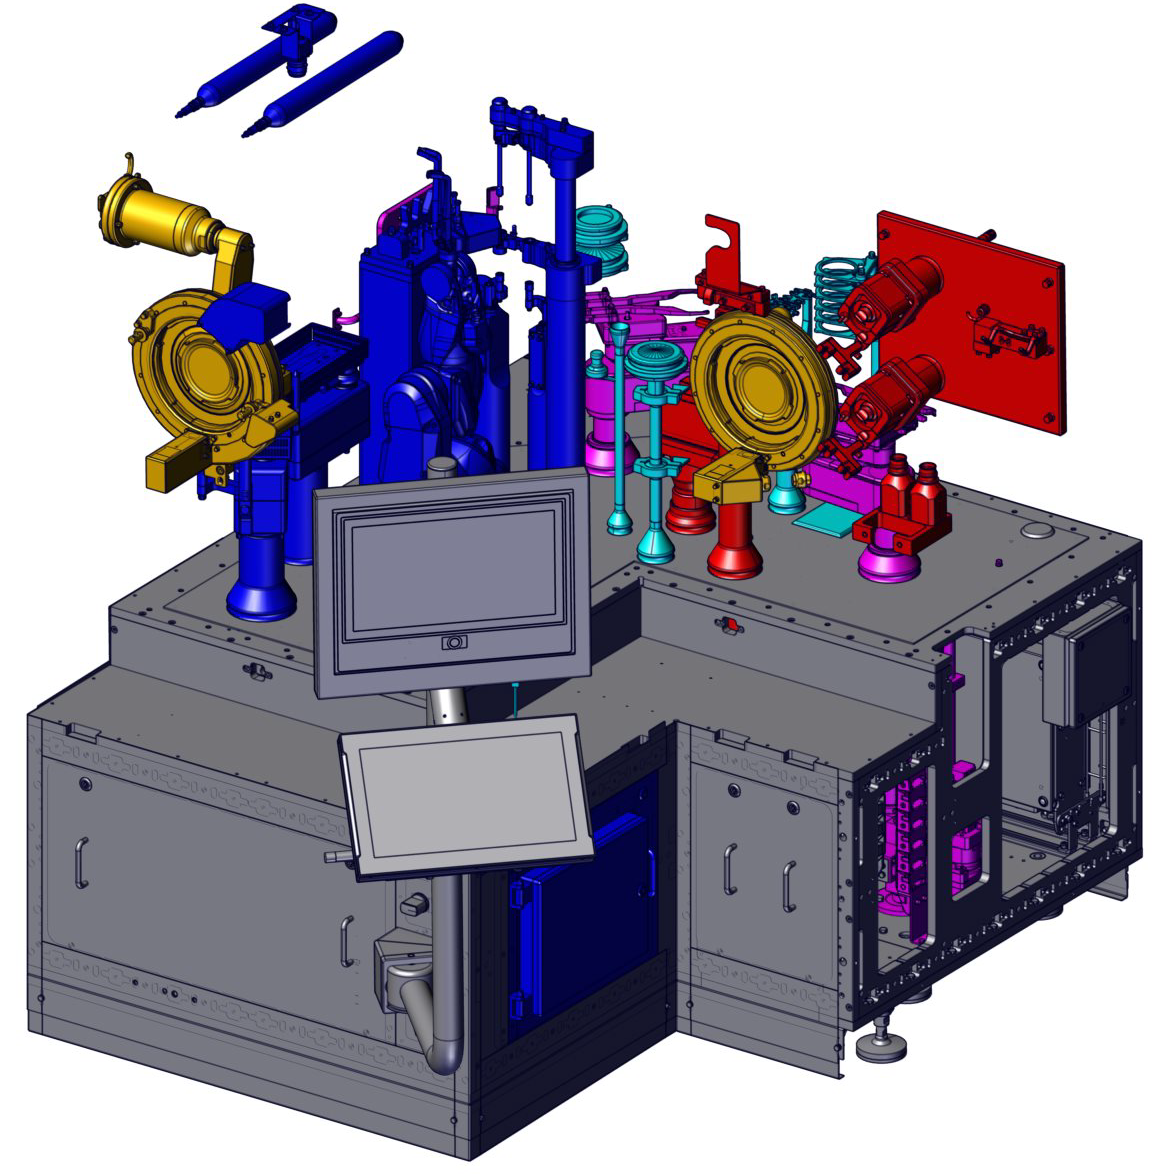
\includegraphics[width=0.5\textwidth]{Bilder/robocell/filling_closing_module.png}
    \caption[robocell Abfüll- und Verschließmodul]{robocell Abfüll- und Verschließmodul (Quelle: \cite{RobocellBetriebsanleitung})}
    \label{fig:robocell}
\end{figure}

\vspace{-0.25em}
\subsection{Technologische Grundlagen}
Im Folgenden werden die technologischen Grundlagen erläutert, die für das Verständnis und die Umsetzung dieser Arbeit besonders relevant sind.
\subsubsection{AASX Package Explorer}
Der AASX Package Explorer, nachfolgend als Package Explorer bezeichnet, wurde als Referenzimplementierung für die \acs{aas} gemäß den Spezifikationen der \acs{idta} entwickelt.
Das Tool ist als Open-Source-Software \cite{AASXPackageExplorer} verfügbar und ermöglicht das Erstellen und Bearbeiten von \acs{aas} im standardisierten AASX-Dateiformat.

Der Package Explorer verfügt dabei über eine benutzerfreundliche grafische Oberfläche (siehe Abbildung \ref{fig:AASXPackageExplorer}), die insbesondere Einsteigern den Zugang zur Modellierung erleichtert.
Dabei können Submodelle, Eigenschaften, semantische Referenzen sowie Metadaten strukturiert definiert und verwaltet werden.
Gleichzeitig bietet der Package Explorer auch erweiterte Funktionen, wie das Erstellen von \acsp{smt}, wodurch er sich auch für den professionellen Einsatz eignet.

Neben der lokalen Modellierung erlaubt das Tool ebenfalls die Verbindung zu einem AAS-Server über standardisierte Schnittstellen (z.B. \acs{opcua} oder \acs{http}/\acs{rest}).
Dies ermöglicht den Betrieb von \acs{aas} in verteilten Systemen.
Besonders geeignet hierfür%
\pagebreak
~ist der Referenzserver des Eclipse-AAS-Projekts \cite{AASXServer}, der das Hosten und Bereitstellen von AASX-Paketen ermöglicht sowie eine nahtlose Integration mit dem Package Explorer erlaubt.

\begin{figure}[htbp]
    \centering
    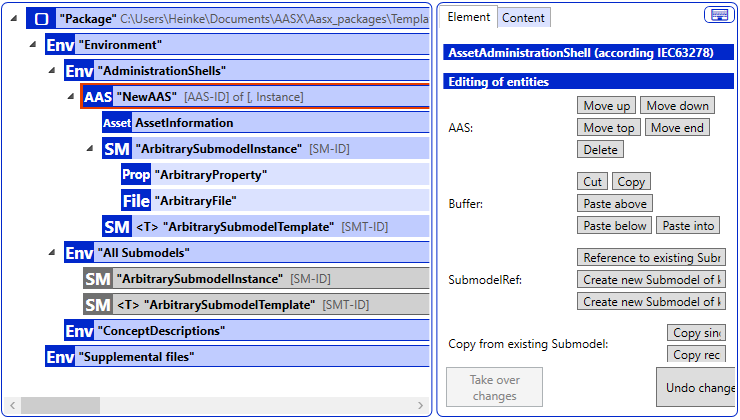
\includegraphics[scale=0.765]{Bilder/ModellierungAAS/Final/Grundlagen_PE.PNG}
    \caption[Benutzeroberfläche Package Explorer]{Benutzeroberfläche Package Explorer} 
    \label{fig:AASXPackageExplorer}
\end{figure}

\subsubsection{Eclipse BaSyx }
Eclipse BaSyx ist eine vom Fraunhofer-Institut für Experimentelles Software Engineering entwickelte Open-Source-Plattform für die Realisierung von Industrie-4.0-Anwendungen.
Mittlerweile wird das Projekt unter dem Dach der Eclipse Foundation weitergeführt.
Der Fokus liegt auf einer einfachen Umsetzung einer Infrastruktur zur Erstellung und Verwaltung digitaler Zwillinge auf Basis der \acs{aas}.
Die Software steht dabei allen Interessenten frei zur Verfügung.

Die Softwarearchitektur basiert auf einer Vielzahl von Standardkomponenten (Off-the-Shelf), die alle als Docker-Container frei zugänglich sind und somit eine nahtlose Integration in bestehende Docker-Umgebungen erlauben.
Eine der wichtigsten Komponenten ist die Registry. 
Sie ist, genau wie alle anderen Komponenten, auf den Spezifikationen der \acs{aas} aufgebaut, insbesondere auf der Spezifikation Part 2: Application Programming Interfaces \cite{SpezifikationPart2}.
In ihr können neue \acs{aas} registriert und bereits vorhandene \acs{aas} anhand ihrer eindeutigen Kennung gesucht werden.
Sie bildet damit die zentrale Anlaufstelle für Geräte und Anwendungen innerhalb des BaSyx-Systems.
Analog dazu existiert eine separate Registry für die Verwaltung von Submodellen.

\newpage
Die eigentlichen Daten werden in der sogenannten \acs{aas} Environment gespeichert und organisiert.
Sie umfasst Repositories für \acs{aas}, Submodelle und Concept Descriptions.
In der Regel ist eine Datenbank, standardmäßig eine MongoDB als persistenter Speicher hinterlegt.
Wie auch alle anderen Komponente stellen diese Repositories standardisierte Schnittstellen basierend auf der \acs{api}-Spezifikation zur Verfügung.
Dies erlaubt z.~B. das Abfragen, Erstellen oder Aktualisieren einer \acs{aas} samt ihrer Submodelle und Inhalte.
Alle verfügbaren Endpunkte dieser Schnittstellen können unter anderem in der automatisch generierten Swagger-Dokumentation eingesehen und ausgeführt werden. 
Typische \acs{rest}-Endpunkte sind beispielsweise:

% \vspace{1em}
{\small
\begin{longtblr}[
  label = tab:aas_endpoints,
  caption = {REST-Endpunkte in Eclipse BaSyx},
  entry = REST-Endpunkte in Eclipse BaSyx
]{
  colspec = {c l X},
  rowhead = 1,
  vlines,
  hlines
}
\textbf{Methode} & \textbf{Endpunkt} & \textbf{Beschreibung} \\
\textcolor{green!50!black}{\textit{GET}} & \texttt{/shells} & Liste aller AAS abrufen \\
\textcolor{green!50!black}{\textit{GET}} & \texttt{/shells/\{aasIdentifier\}} & Bestimmte AAS anzeigen \\
\textcolor{green!50!black}{\textit{GET}} & \texttt{/submodels} & Liste aller Submodelle aufrufen \\
\textcolor{orange!85!black}{\textit{POST}} & \texttt{/shells} & Neue AAS erstellen \\
\textcolor{orange!85!black}{\textit{POST}} & \texttt{/submodels} & Neues Submodell erstellen \\
\textcolor{red!80!black}{\textit{DELETE}} & \texttt{/shells/\{aasIdentifier\}} & AAS löschen \\
\end{longtblr}
}
\vspace{-0.5em}

Im BaSyx-System ermöglicht ein Discovery Service die Verknüpfung physischer Assets mit iheren zugehörigen \acs{aas}.
Dies ist insbesondere für die Abbildung von hierarchischen Strukturen wie Stücklisten (\ac{bom}) von großer Bedeutung.
Ein übergeordnetes Asset (z.B. Maschine) kann so beispielsweise mit untergeordneten Komponenten (z.B. Antrieb, Sensoren) logisch über deren AAS verbunden werden.
Einträge in den Discovery Service müssen derzeit allerdings noch manuell über die \acs{api} (Aplication Programming Interface) vorgenommen werden.

Zur benutzerfreundlichen Visualisierung und Interaktion kann die sogenannte AAS Web UI genutzt werden.
Die webbasierte Benutzeroberfläche, wie in Abbildung \ref{fig:BasyxWebUI} dargestellt ist, wurde mit dem JavaScript-Framework Vue.js entwickelt und kommuniziert über die standardisierte \acs{rest}-API mit den zentralen Komponenten der BaSyx-Plattform, darunter die Repositories, Registries und der Discovery Service.
Sie zeigt alle registrierten \acs{aas} in einer Liste an und bietet die Möglichkeit, einzelne \acs{aas} in einer Baumstruktur sowohl zu visualisieren als auch zu bearbeiten. 

Ein weiteres zentrales Merkmal der AAS Web UI ist der sogenannte AAS Viewer.
In nachfolgender Abbildung ist dieser auf der rechten Seite angeordnet.
Er erlaubt die Visualisierung von Submodellen und deren Elementen anhand ihrer semanticId. 
Hierfür stehen verschiedene vordefinierte Plugins zur Verfügung, die bestimmte Submodelle, wie beispielsweise das Typenschild oder hierarchische Strukturen, grafisch darstellen.
Da die Lösung Open Source ist besteht zudem die Möglichkeit, eigene benutzerdefinierte Plugins für weitere Submodelle zu erstellen. \cite{BaSyxWiki} \cite{BaSyxEclipse}

\vspace{0.5em}
\begin{figure}[htbp]
    \centering
    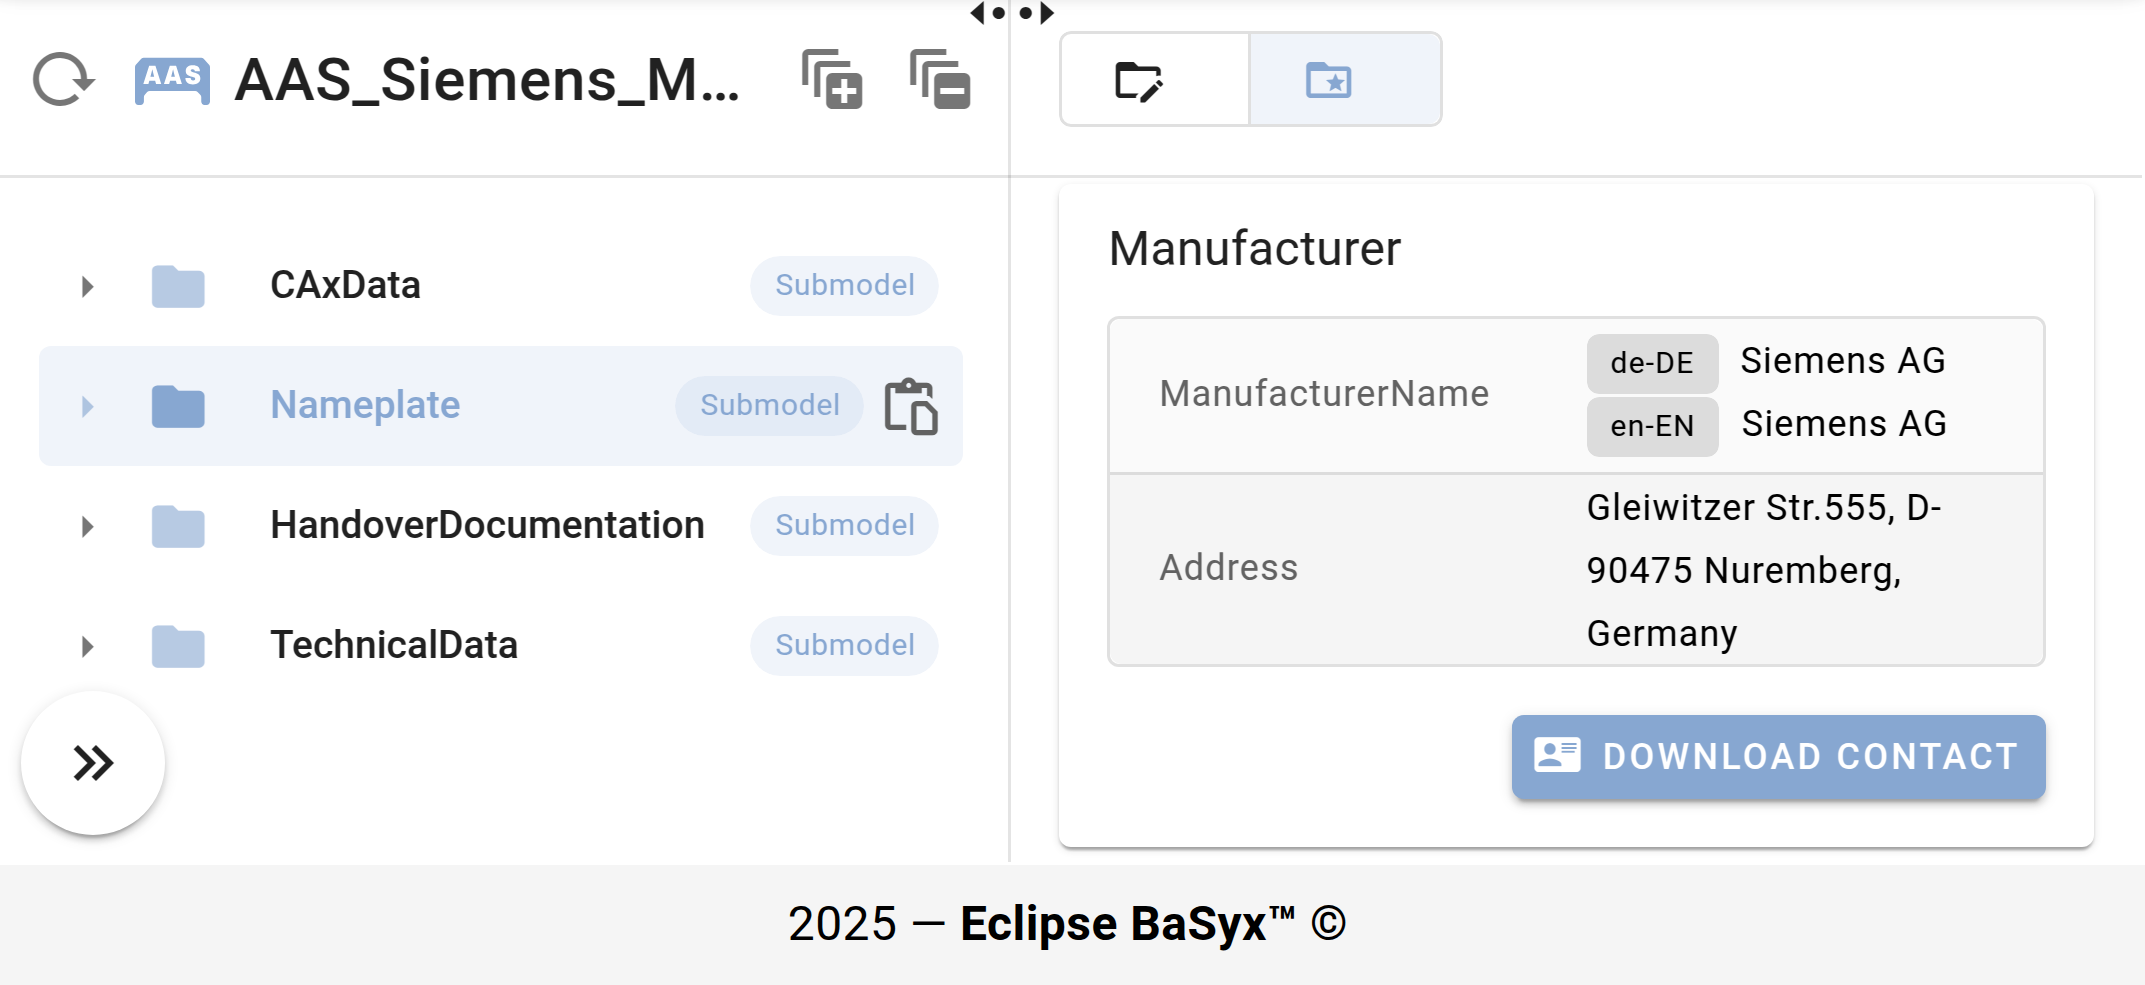
\includegraphics[width=1\textwidth]{Bilder/AASWebUZIGrundlagen.png}
    \caption[Benutzeroberfläche AAS Web UI]{Benutzeroberfläche AAS Web UI}
    \label{fig:BasyxWebUI}
\end{figure}


\subsubsection{OPC Unified Architecture}
\acs{opcua} ist ein plattformübergreifender Kommunikationsstandard, der speziell für die Anforderungen der industriellen Automatisierung entwickelt wurde.
Ziel ist ein herstellerübergreifender, sicherer und standardisierter Datenaustausch.
In \acs{rami} \cite{RAMI4.0} wird \acs{opcua} als empfohlener Standard für die Kommunikationsschicht definiert und bildet damit die Grundlage für die Interoperabilität zwischen Maschinen, Anlagen und IT-Systemen verschiedener Hersteller.

Die grundlegende Idee von \acs{opcua} besteht darin, dass ein Maschinenhersteller einen \acs{opcua} Server bereitstellt, der einen standardisierten und herstellerunabhängigen Zugriff auf eine Maschine ermöglicht.
Der Server dient hierbei als zentrale Schnittstelle zur Außenwelt. Er implementiert den OPC Standard und stellt strukturierte Informationen sowie Zugriffsmöglichkeiten auf Maschinenzustände und -daten bereit.
Im Inneren kommuniziert der Server dabei über ein herstellerspezifisches, proprietäres Protokoll mit der Steuerung.
Zum Auslesen oder Austauschen dieser Daten wird ein \acs{opcua} Client benötigt. Dieser agiert als Kommunikationspartner des Servers, stellt die Verbindung her und ermöglicht den bidirektionalen Datentransfer. \cite{OPCUA}